\documentclass{standalone}
\usepackage{tikz}
\usetikzlibrary{patterns, positioning}

\begin{document}
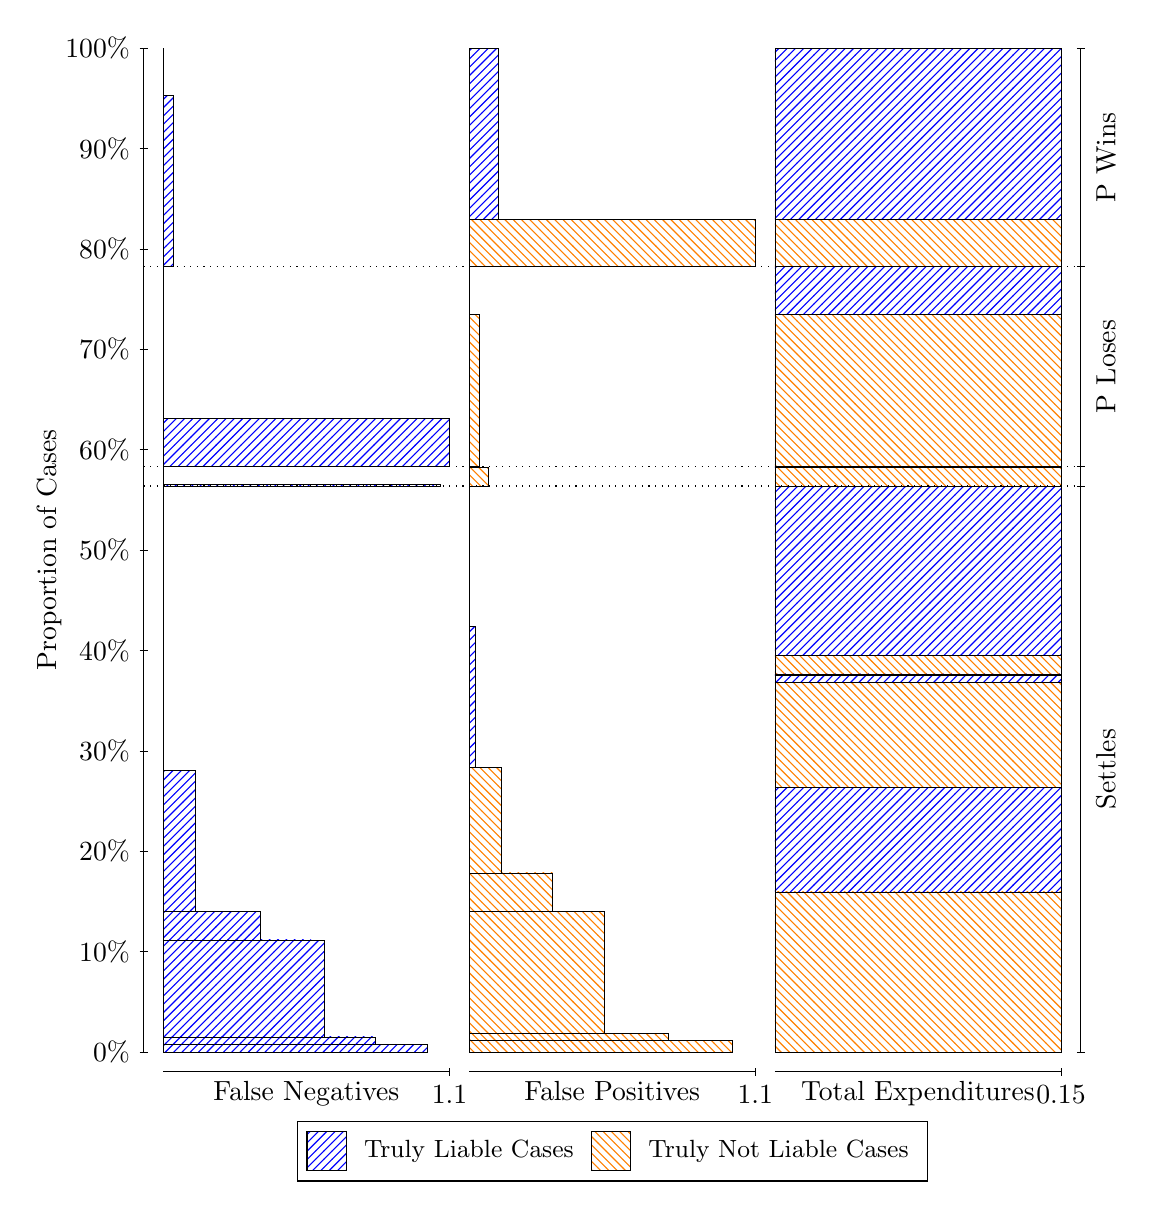
\begin{tikzpicture}
\draw[black, very thin] (1.5,1.75) -- (1.5,14.5);
\node[rotate=90, anchor=center] at (0.3, 8.125) {Proportion of Cases};
\draw[black, very thin] (1.45,1.75) -- (1.55,1.75);
\node[anchor=east] at (1.45, 1.75) {0\%};
\draw[black, very thin] (1.45,3.025) -- (1.55,3.025);
\node[anchor=east] at (1.45, 3.025) {10\%};
\draw[black, very thin] (1.45,4.3) -- (1.55,4.3);
\node[anchor=east] at (1.45, 4.3) {20\%};
\draw[black, very thin] (1.45,5.575) -- (1.55,5.575);
\node[anchor=east] at (1.45, 5.575) {30\%};
\draw[black, very thin] (1.45,6.85) -- (1.55,6.85);
\node[anchor=east] at (1.45, 6.85) {40\%};
\draw[black, very thin] (1.45,8.125) -- (1.55,8.125);
\node[anchor=east] at (1.45, 8.125) {50\%};
\draw[black, very thin] (1.45,9.4) -- (1.55,9.4);
\node[anchor=east] at (1.45, 9.4) {60\%};
\draw[black, very thin] (1.45,10.675) -- (1.55,10.675);
\node[anchor=east] at (1.45, 10.675) {70\%};
\draw[black, very thin] (1.45,11.95) -- (1.55,11.95);
\node[anchor=east] at (1.45, 11.95) {80\%};
\draw[black, very thin] (1.45,13.225) -- (1.55,13.225);
\node[anchor=east] at (1.45, 13.225) {90\%};
\draw[black, very thin] (1.45,14.5) -- (1.55,14.5);
\node[anchor=east] at (1.45, 14.5) {100\%};

\draw[black, very thin] (13.4,1.75) -- (13.4,14.5);
\draw[black, very thin] (13.35,1.75) -- (13.45,1.75);
\node[anchor=west] at (13.35, 1.75) {};
\draw[black, very thin] (13.35,8.9378) -- (13.45,8.9378);
\node[anchor=west] at (13.35, 8.9378) {};
\draw[black, very thin] (13.35,9.19) -- (13.45,9.19);
\node[anchor=west] at (13.35, 9.19) {};
\draw[black, very thin] (13.35,11.722) -- (13.45,11.722);
\node[anchor=west] at (13.35, 11.722) {};
\draw[black, very thin] (13.35,14.5) -- (13.45,14.5);
\node[anchor=west] at (13.35, 14.5) {};

\draw[black, very thin, pattern color=blue, pattern=north east lines] (1.75,1.75) rectangle (5.0976,1.846);
\draw[black, very thin, pattern color=blue, pattern=north east lines] (1.75,1.846) rectangle (4.4444,1.9407);
\draw[black, very thin, pattern color=blue, pattern=north east lines] (1.75,1.9407) rectangle (3.7912,3.168);
\draw[black, very thin, pattern color=blue, pattern=north east lines] (1.75,3.168) rectangle (3.6279,3.1747);
\draw[black, very thin, pattern color=blue, pattern=north east lines] (1.75,3.1747) rectangle (2.9747,3.5341);
\draw[black, very thin, pattern color=blue, pattern=north east lines] (1.75,3.5341) rectangle (2.1582,5.3275);
\draw[black, very thin, pattern color=orange, pattern=north west lines] (1.75,5.3275) rectangle (1.75,8.9378);
\draw[black, very thin, pattern color=blue, pattern=north east lines] (1.75,8.9378) rectangle (5.2609,8.9571);
\draw[black, very thin, pattern color=orange, pattern=north west lines] (1.75,8.9571) rectangle (1.75,9.19);
\draw[black, very thin, pattern color=blue, pattern=north east lines] (1.75,9.19) rectangle (5.3833,9.7962);
\draw[black, very thin, pattern color=orange, pattern=north west lines] (1.75,9.7962) rectangle (1.75,11.722);
\draw[black, very thin, pattern color=blue, pattern=north east lines] (1.75,11.722) rectangle (1.8725,13.894);
\draw[black, very thin, pattern color=orange, pattern=north west lines] (1.75,13.894) rectangle (1.75,14.5);
\draw[black, very thin, pattern color=orange, pattern=north west lines] (5.6333,1.75) rectangle (8.9809,1.8933);
\draw[black, very thin, pattern color=orange, pattern=north west lines] (5.6333,1.8933) rectangle (8.1644,1.9842);
\draw[black, very thin, pattern color=orange, pattern=north west lines] (5.6333,1.9842) rectangle (7.5112,1.991);
\draw[black, very thin, pattern color=orange, pattern=north west lines] (5.6333,1.991) rectangle (7.3479,3.5374);
\draw[black, very thin, pattern color=orange, pattern=north west lines] (5.6333,3.5374) rectangle (6.6948,4.0254);
\draw[black, very thin, pattern color=orange, pattern=north west lines] (5.6333,4.0254) rectangle (6.0416,5.3603);
\draw[black, very thin, pattern color=blue, pattern=north east lines] (5.6333,5.3603) rectangle (5.715,7.1537);
\draw[black, very thin, pattern color=blue, pattern=north east lines] (5.6333,7.1537) rectangle (5.6333,8.9378);
\draw[black, very thin, pattern color=orange, pattern=north west lines] (5.6333,8.9378) rectangle (5.8783,9.1707);
\draw[black, very thin, pattern color=blue, pattern=north east lines] (5.6333,9.1707) rectangle (5.6333,9.19);
\draw[black, very thin, pattern color=orange, pattern=north west lines] (5.6333,9.19) rectangle (5.7558,11.116);
\draw[black, very thin, pattern color=blue, pattern=north east lines] (5.6333,11.116) rectangle (5.6333,11.722);
\draw[black, very thin, pattern color=orange, pattern=north west lines] (5.6333,11.722) rectangle (9.2667,12.328);
\draw[black, very thin, pattern color=blue, pattern=north east lines] (5.6333,12.328) rectangle (6.0007,14.5);
\draw[black, very thin, pattern color=orange, pattern=north west lines] (9.5167,1.75) rectangle (13.15,3.7843);
\draw[black, very thin, pattern color=blue, pattern=north east lines] (9.5167,3.7843) rectangle (13.15,5.1063);
\draw[black, very thin, pattern color=orange, pattern=north west lines] (9.5167,5.1063) rectangle (13.15,6.4412);
\draw[black, very thin, pattern color=blue, pattern=north east lines] (9.5167,6.4412) rectangle (13.15,6.5372);
\draw[black, very thin, pattern color=orange, pattern=north west lines] (9.5167,6.5372) rectangle (13.15,6.5441);
\draw[black, very thin, pattern color=blue, pattern=north east lines] (9.5167,6.5441) rectangle (13.15,6.5507);
\draw[black, very thin, pattern color=orange, pattern=north west lines] (9.5167,6.5507) rectangle (13.15,6.7849);
\draw[black, very thin, pattern color=blue, pattern=north east lines] (9.5167,6.7849) rectangle (13.15,8.9378);
\draw[black, very thin, pattern color=orange, pattern=north west lines] (9.5167,8.9378) rectangle (13.15,9.1707);
\draw[black, very thin, pattern color=blue, pattern=north east lines] (9.5167,9.1707) rectangle (13.15,9.19);
\draw[black, very thin, pattern color=orange, pattern=north west lines] (9.5167,9.19) rectangle (13.15,11.116);
\draw[black, very thin, pattern color=blue, pattern=north east lines] (9.5167,11.116) rectangle (13.15,11.722);
\draw[black, very thin, pattern color=orange, pattern=north west lines] (9.5167,11.722) rectangle (13.15,12.328);
\draw[black, very thin, pattern color=blue, pattern=north east lines] (9.5167,12.328) rectangle (13.15,14.5);
\draw[black, dotted] (1.5,8.9378) -- (13.4,8.9378);
\draw[black, dotted] (1.5,9.19) -- (13.4,9.19);
\draw[black, dotted] (1.5,11.722) -- (13.4,11.722);
\draw[black, very thin] (1.75,1.5) -- (5.3833,1.5);
\node[anchor=north] at (3.5667, 1.5) {False Negatives};
\draw[black, very thin] (5.3833,1.45) -- (5.3833,1.55);
\node[anchor=north] at (5.3833, 1.45) {1.1};

\draw[black, very thin] (5.6333,1.5) -- (9.2667,1.5);
\node[anchor=north] at (7.45, 1.5) {False Positives};
\draw[black, very thin] (9.2667,1.45) -- (9.2667,1.55);
\node[anchor=north] at (9.2667, 1.45) {1.1};

\draw[black, very thin] (9.5167,1.5) -- (13.15,1.5);
\node[anchor=north] at (11.333, 1.5) {Total Expenditures};
\draw[black, very thin] (13.15,1.45) -- (13.15,1.55);
\node[anchor=north] at (13.15, 1.45) {0.15};

\node[black, centered, rotate=90] at (13.72, 5.3439) {Settles};

\node[black, centered, rotate=90] at (13.72, 10.456) {P Loses};
\node[black, centered, rotate=90] at (13.72, 13.111) {P Wins};

\draw (7.449999999999999,1.5) node[draw=none] (baseCoordinate) {};
\begin{scope}[align=center]
        \matrix[scale=0.5, draw=black, below=0.5cm of baseCoordinate, nodes={draw}, column sep=0.1cm]{
            \node[rectangle, draw, minimum width=0.5cm, minimum height=0.5cm, pattern=north east lines, pattern color=blue] {}; &
            \node[draw=none, font=\small] (B) {Truly Liable Cases}; &
            \node[rectangle, draw, minimum width=0.5cm, minimum height=0.5cm, pattern=north west lines, pattern color=orange] {}; &
            \node[draw=none, font=\small] (B) {Truly Not Liable Cases}; \\
            };
\end{scope}

\end{tikzpicture}
\end{document}